\pdfminorversion=4
\documentclass[aspectratio=169]{beamer}

\mode<presentation>
{
  \usetheme{default}
  \usecolortheme{default}
  \usefonttheme{default}
  \setbeamertemplate{navigation symbols}{}
  \setbeamertemplate{caption}[numbered]
  \setbeamertemplate{footline}[frame number]  % or "page number"
  \setbeamercolor{frametitle}{fg=white}
  \setbeamercolor{footline}{fg=black}
} 

\usepackage[english]{babel}
\usepackage{inputenc}
\usepackage{tikz}
\usepackage{courier}
\usepackage{array}
\usepackage{bold-extra}
\usepackage{minted}
\usepackage[thicklines]{cancel}
\usepackage{fancyvrb}
\usepackage{colortbl}

\xdefinecolor{dianablue}{rgb}{0.18,0.24,0.31}
\xdefinecolor{darkblue}{rgb}{0.1,0.1,0.7}
\xdefinecolor{darkgreen}{rgb}{0,0.5,0}
\xdefinecolor{darkgrey}{rgb}{0.35,0.35,0.35}
\xdefinecolor{darkorange}{rgb}{0.8,0.5,0}
\xdefinecolor{darkred}{rgb}{0.7,0,0}
\definecolor{darkgreen}{rgb}{0,0.6,0}
\definecolor{mauve}{rgb}{0.58,0,0.82}

\title[2024-10-21-chep2024-hep-help]{\vspace{0.5 cm} \\ HEP-Help: a first-stop helpline for particle physics software \\ \vspace{-0.75 cm}\hspace{7 cm}\uncover<2->{
\includegraphics[height=2 cm]{PLOTS/in-progress.png}}\vspace{-1.75 cm}}
\author{Jim Pivarski}
\institute{Princeton University -- IRIS-HEP}
\date{October 21, 2024}

\usetikzlibrary{shapes.callouts}

\usepackage{array}
\newcolumntype{L}[1]{>{\raggedright\let\newline\\\arraybackslash\hspace{0pt}}p{#1}}
\newcolumntype{C}[1]{>{\centering\let\newline\\\arraybackslash\hspace{0pt}}p{#1}}

\begin{document}

\logo{\pgfputat{\pgfxy(0.11, 7.4)}{\pgfbox[right,base]{\tikz{\filldraw[fill=dianablue, draw=none] (0 cm, 0 cm) rectangle (50 cm, 1 cm);}\mbox{\hspace{-8 cm}
\includegraphics[height=1 cm]{princeton-logo-long.png}\hspace{0.1 cm}\raisebox{0.1 cm}{
\includegraphics[height=0.8 cm]{iris-hep-logo-long.png}}\hspace{0.1 cm}}}}}

\begin{frame}
  \titlepage
\end{frame}

\logo{\pgfputat{\pgfxy(0.11, 7.4)}{\pgfbox[right,base]{\tikz{\filldraw[fill=dianablue, draw=none] (0 cm, 0 cm) rectangle (50 cm, 1 cm);}\mbox{\hspace{-8 cm}
\includegraphics[height=1 cm]{princeton-logo.png}\hspace{0.1 cm}\raisebox{0.1 cm}{
\includegraphics[height=0.8 cm]{iris-hep-logo.png}}\hspace{0.1 cm}}}}}

% Uncomment these lines for an automatically generated outline.
%\begin{frame}{Outline}
%  \tableofcontents
%\end{frame}

% START START START START START START START START START START START START START

\begin{frame}{For a long time, I've wanted a ``StackOverflow for HEP''}
\large
\vspace{0.5 cm}
\begin{columns}[t]
\column{0.33\linewidth}
\textcolor{darkblue}{PyHEP 2019:} I tried to get everybody to {\it use} StackOverflow, with tags to carve out our space within it.

\vspace{0.25 cm}
\fbox{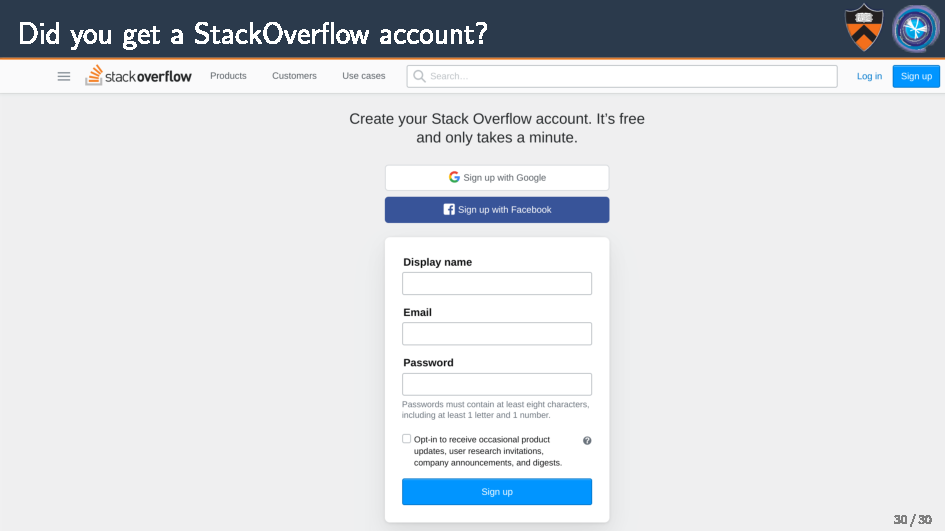
\includegraphics[width=\linewidth]{PLOTS/2019_10_17_pyhep_awkward-slide.pdf}}

%% \small
%% \vspace{0.25 cm}
%% \uncover<2->{\textcolor{gray}{(Creating our own StackExchange site would be a bigger community effort.)}}

\column{0.33\linewidth}
\uncover<2->{\textcolor{darkblue}{JLab Future Trends 2022:} I acknowledged that it's not going well.}

\vspace{0.25 cm}
\uncover<2->{\fbox{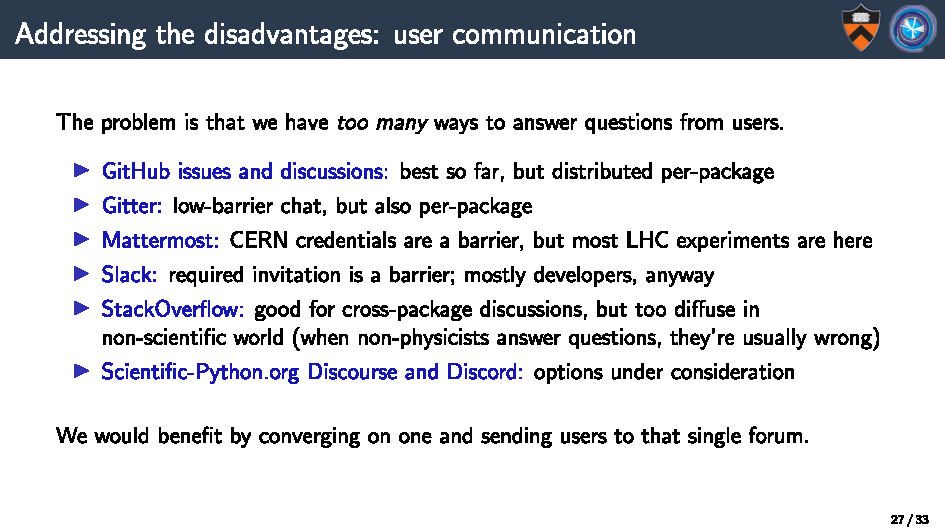
\includegraphics[width=\linewidth]{PLOTS/2022_09_28_future_trends_python-slide.pdf}}}

%% \small
%% \vspace{0.25 cm}
%% \uncover<4->{\textcolor{gray}{(Despite the tags, StackOverflow questions get more answers from general programmers who don't recognize the need for scaling.)}}

\column{0.33\linewidth}
\uncover<3->{\textcolor{darkblue}{Analysis Ecosystem II 2022} and \textcolor{darkblue}{PyHEP.dev 2023:} Brainstorming sessions, never landed on a solution.}

\vspace{0.25 cm}
\uncover<3->{\fbox{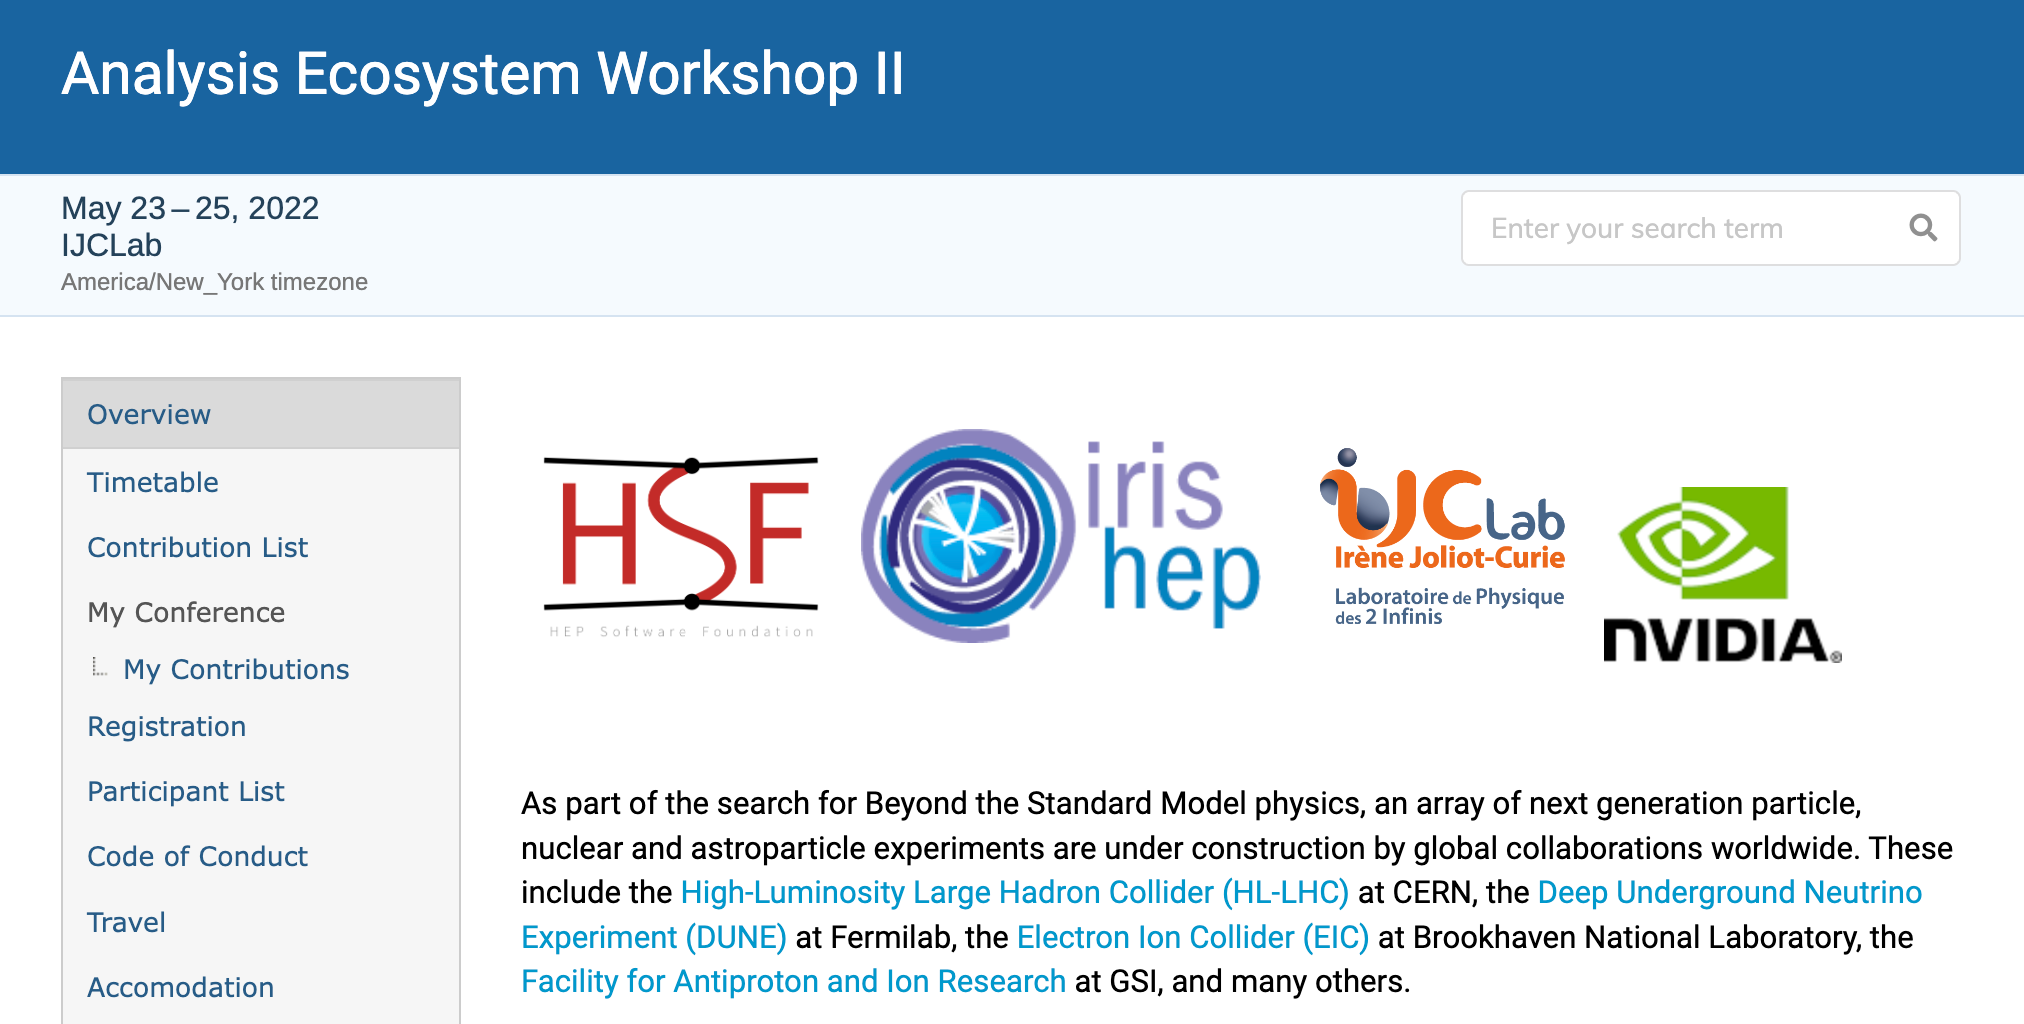
\includegraphics[width=\linewidth]{PLOTS/2022-05-23-analysis-ecosystem-ii-banner.png}}}

\vspace{0.25 cm}
\uncover<3->{\fbox{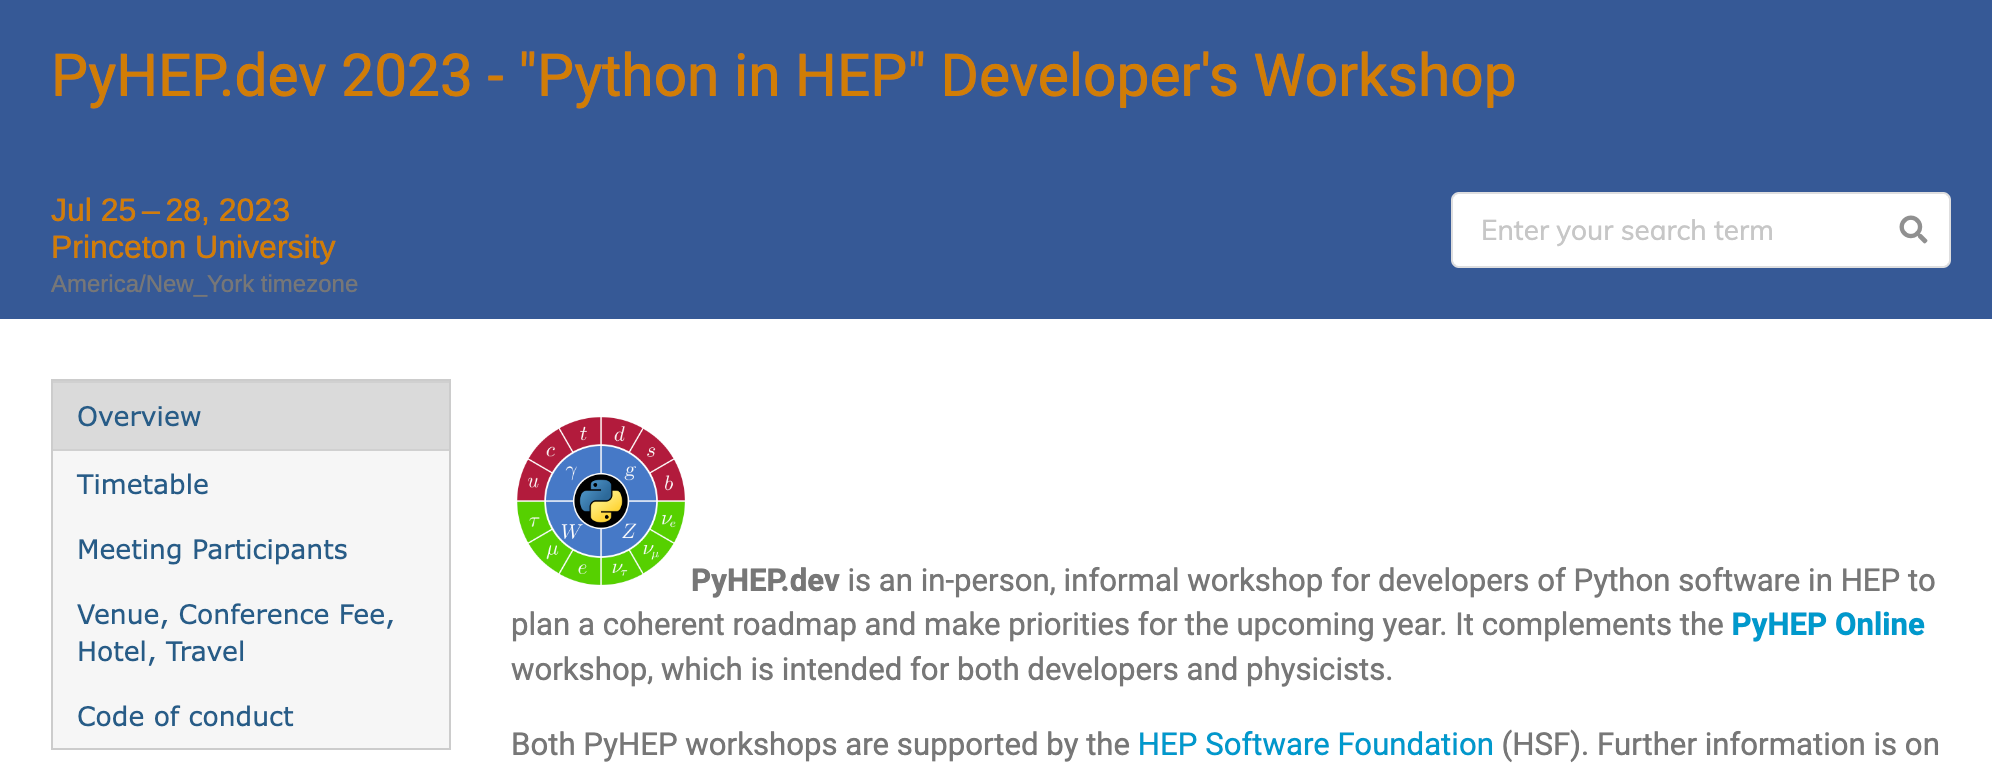
\includegraphics[width=\linewidth]{PLOTS/2023-07-25-pyhepdev-banner.png}}}

\end{columns}
\end{frame}

\begin{frame}{The current state of user-help across HEP software packages}
\vspace{0.25 cm}
\begin{center}
\fbox{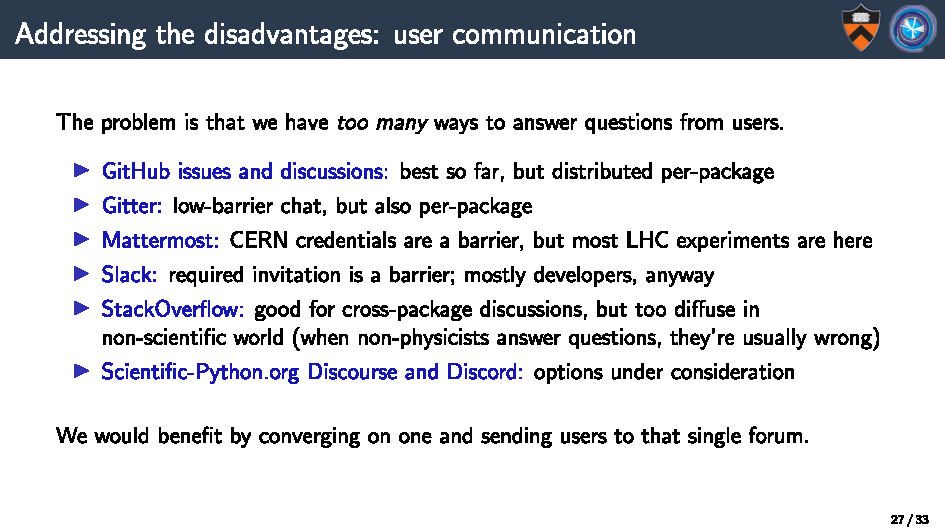
\includegraphics[width=0.9\linewidth]{PLOTS/2022_09_28_future_trends_python-slide.pdf}}
\end{center}
\end{frame}

\begin{frame}{The ROOT Forum does not have this problem}
\large
\vspace{0.25 cm}

\begin{center}
\fbox{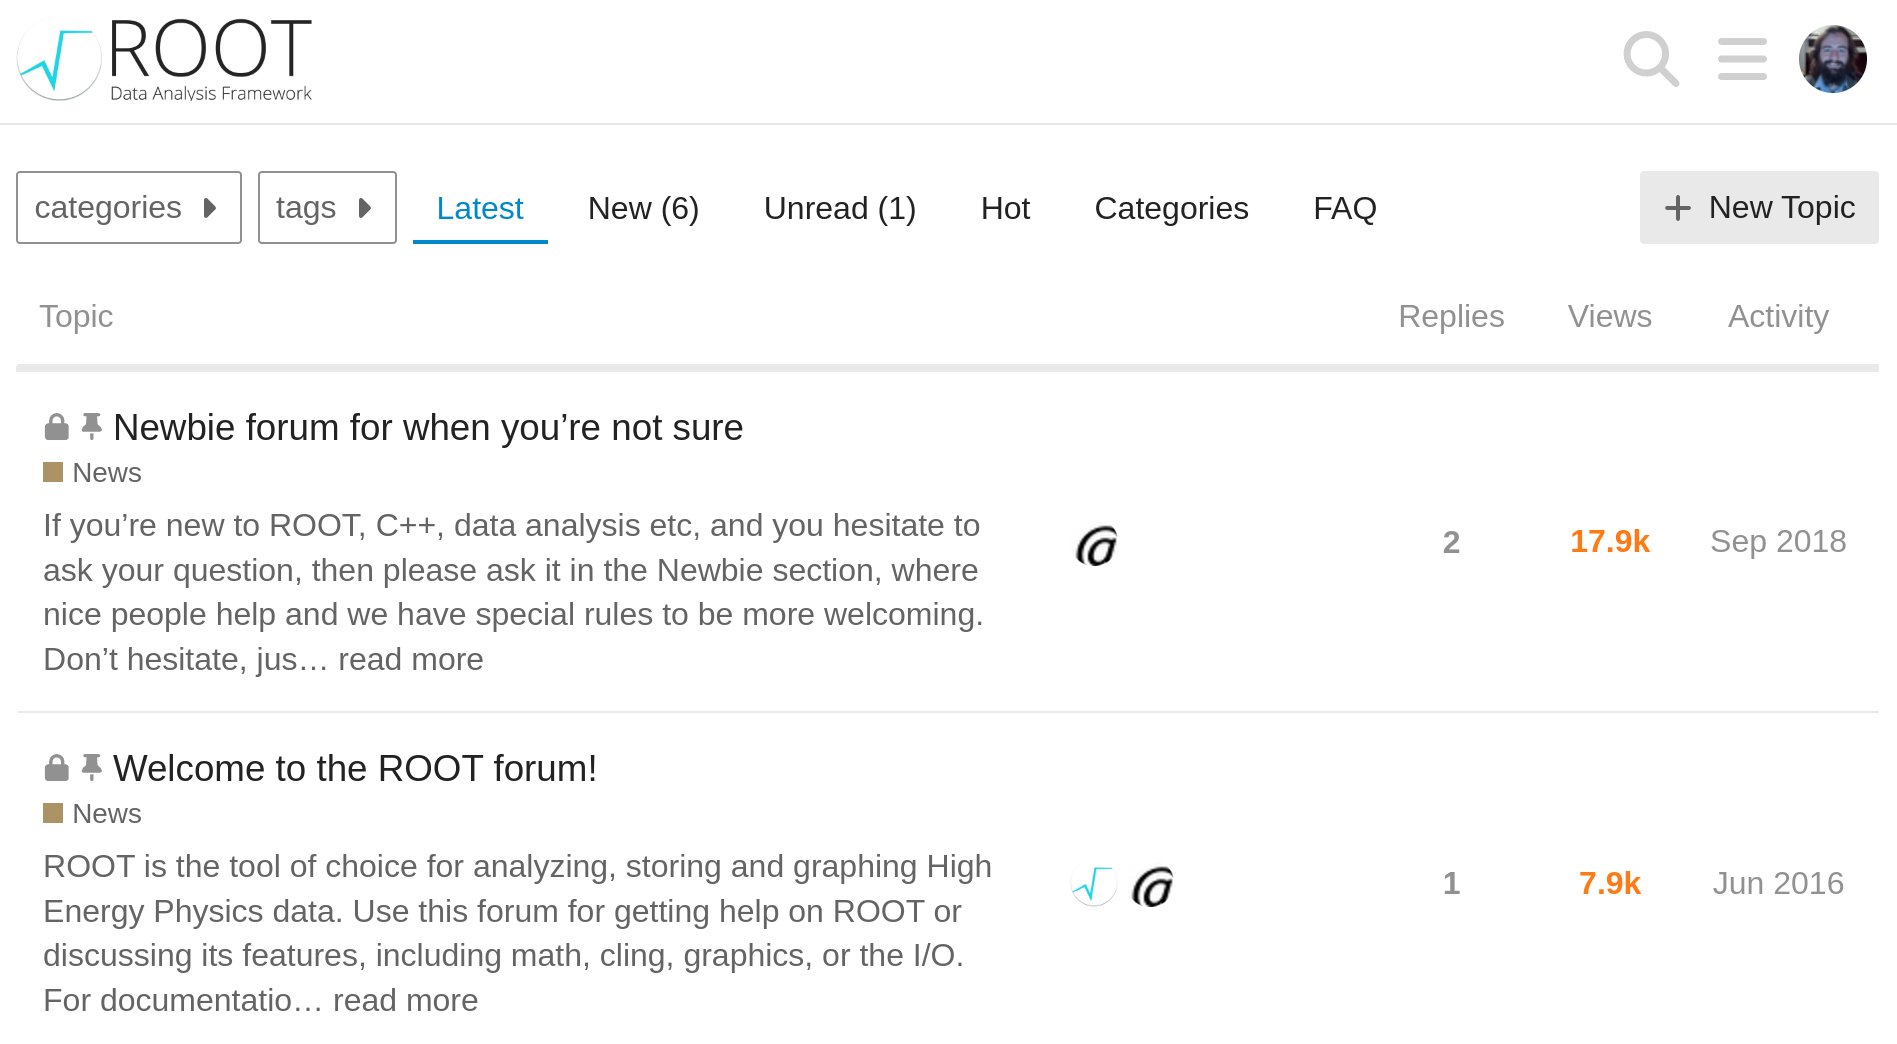
\includegraphics[width=0.7\linewidth]{PLOTS/root-forum-banner.png}}
\end{center}

\begin{itemize}
\item<2-> It's easy for newcomers to find, and ROOT team ensures that there's always someone ``on shift'' to answer questions.
\item<3-> Deep historical archive of past questions and answers.
\end{itemize}
\end{frame}

\begin{frame}{\mbox{ }}
\large
\vspace{0.5 cm}
Similarly, IRIS-HEP Slack, Coffea Users in CMS Mattermost, and some GitHub Discussions are very active.

\vspace{1 cm}
\uncover<2->{Moving active communities is hard, and runs the risk of dispersing them instead.}

\vspace{1 cm}
\begin{uncoverenv}<3->
\textcolor{darkblue}{Better strategy:} make an entry point that

\vspace{0.25 cm}
\begin{itemize}
\item shows people where a question has already been answered
\item leads people to the right place to engage with already-active communities.
\end{itemize}
\end{uncoverenv}
\end{frame}

\begin{frame}{New monkey wrench}
\vspace{0.17 cm}
\begin{columns}
\column{1.15\linewidth}
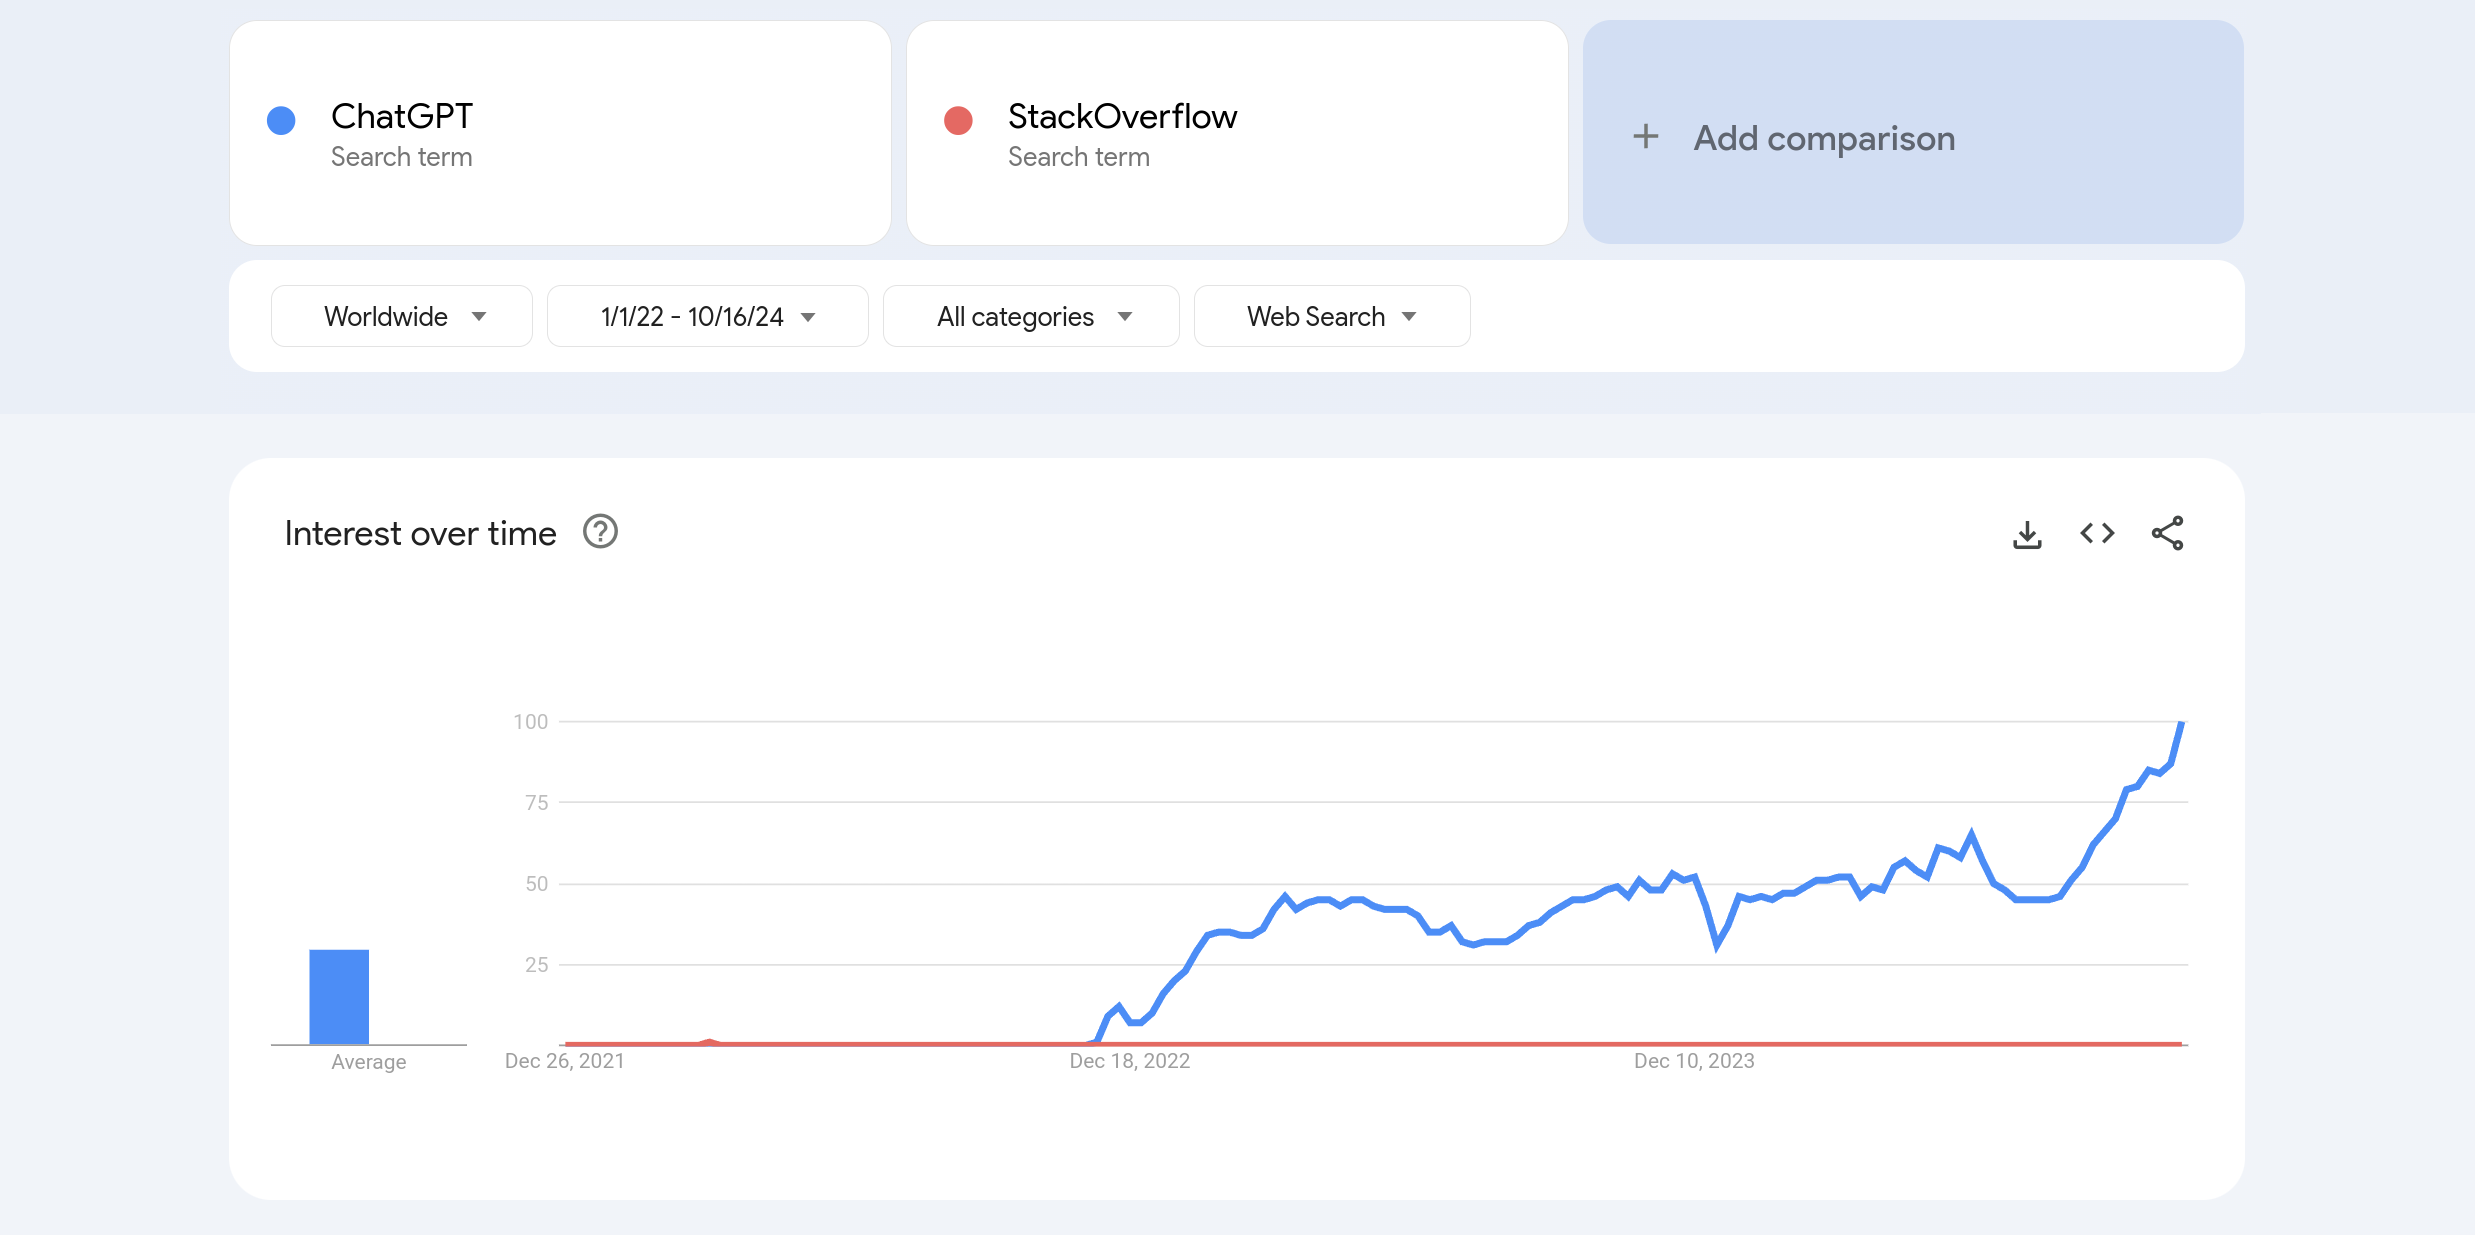
\includegraphics[width=\linewidth]{PLOTS/googletrends-chatgpt.png}
\end{columns}
\end{frame}

\begin{frame}{\mbox{ }}
\Large
\vspace{1 cm}

Can a Large Language Model (LLM) be a first responder, either to answer questions or to send people to a forum where their question can be answered or has already been answered?

\vspace{0.5 cm}
\begin{center}
\uncover<2->{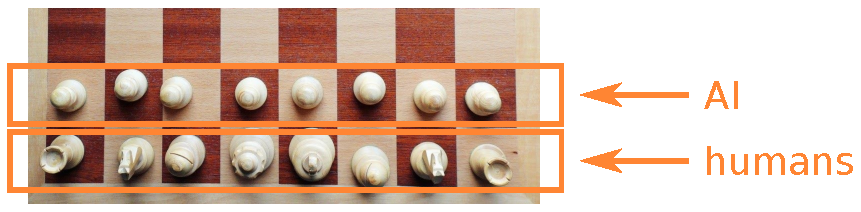
\includegraphics[width=0.8\linewidth]{PLOTS/ai-humans-chess-metaphor.pdf}}
\end{center}
\end{frame}

\begin{frame}{LLMs for HEP is a popular topic this year!}
\small
\vspace{0.25 cm}
\begin{columns}
\column{1.1\linewidth}\renewcommand{\arraystretch}{1.04}
\begin{tabular}{C{0.15\linewidth} L{0.34\linewidth} L{0.18\linewidth} C{0.07\linewidth} C{0.12\linewidth}}\arrayrulecolor{gray}
RAG/search & \textcolor{blue}{\href{https://indico.cern.ch/event/1338689/contributions/6011147/}{Leveraging Language Models to Navigate Conference Abstracts: An Open-Source Approach}} & Gordon Watts & talk & next talk, here \\\hline
RAG/search & \textcolor{blue}{\href{https://indico.cern.ch/event/1338689/contributions/6010661/}{AccGPT: A CERN Knowledge Retrieval Chatbot}} & Florian Rehm, Juan Guijarro, Sofia Vallecorsa, Verena Kain & talk & 20 minutes ago, rm 2A \\\hline
RAG/search & \textcolor{blue}{\href{https://indico.cern.ch/event/1338689/contributions/6010735/}{Docu-Bot: AI assisted user support}} & Jiri Chudoba & poster & maybe still up, Lobby \\\hline
code review & \textcolor{blue}{\href{https://indico.cern.ch/event/1338689/contributions/6010676/}{Leveraging Language Models for Enhanced Code Review in Particle Physics Software Development}} & Alexey Rybalchenko & poster & Tue 3pm, rm 4 \\\hline
domain-specific chat-bot & \textcolor{blue}{\href{https://indico.cern.ch/event/1338689/contributions/6010731/}{Xiwu: A basic flexible and learnable LLM for High Energy Physics}} & Ke Li, Siyang Chen, Yiyu Zhang, Zhengde Zhang & poster & Tue 3pm, rm 4 \\\hline
domain-specific chat-bot & \textcolor{blue}{\href{https://indico.cern.ch/event/1338689/contributions/6010732/}{Boost physics study at HEP experiments with Dr. Sai}} & {\it same authors} + Yipu Liao & poster & Tue 3pm, rm 4 \\\hline
general & \textcolor{blue}{\href{https://indico.cern.ch/event/1338689/contributions/6066662/}{Large Language Models in Physics}} & Sarah Heim & plenary & Tue 11am \\
\end{tabular}
\end{columns}
\end{frame}

\begin{frame}{One more, not at CHEP: chATLAS}
\vspace{0.2 cm}
\begin{center}
\fbox{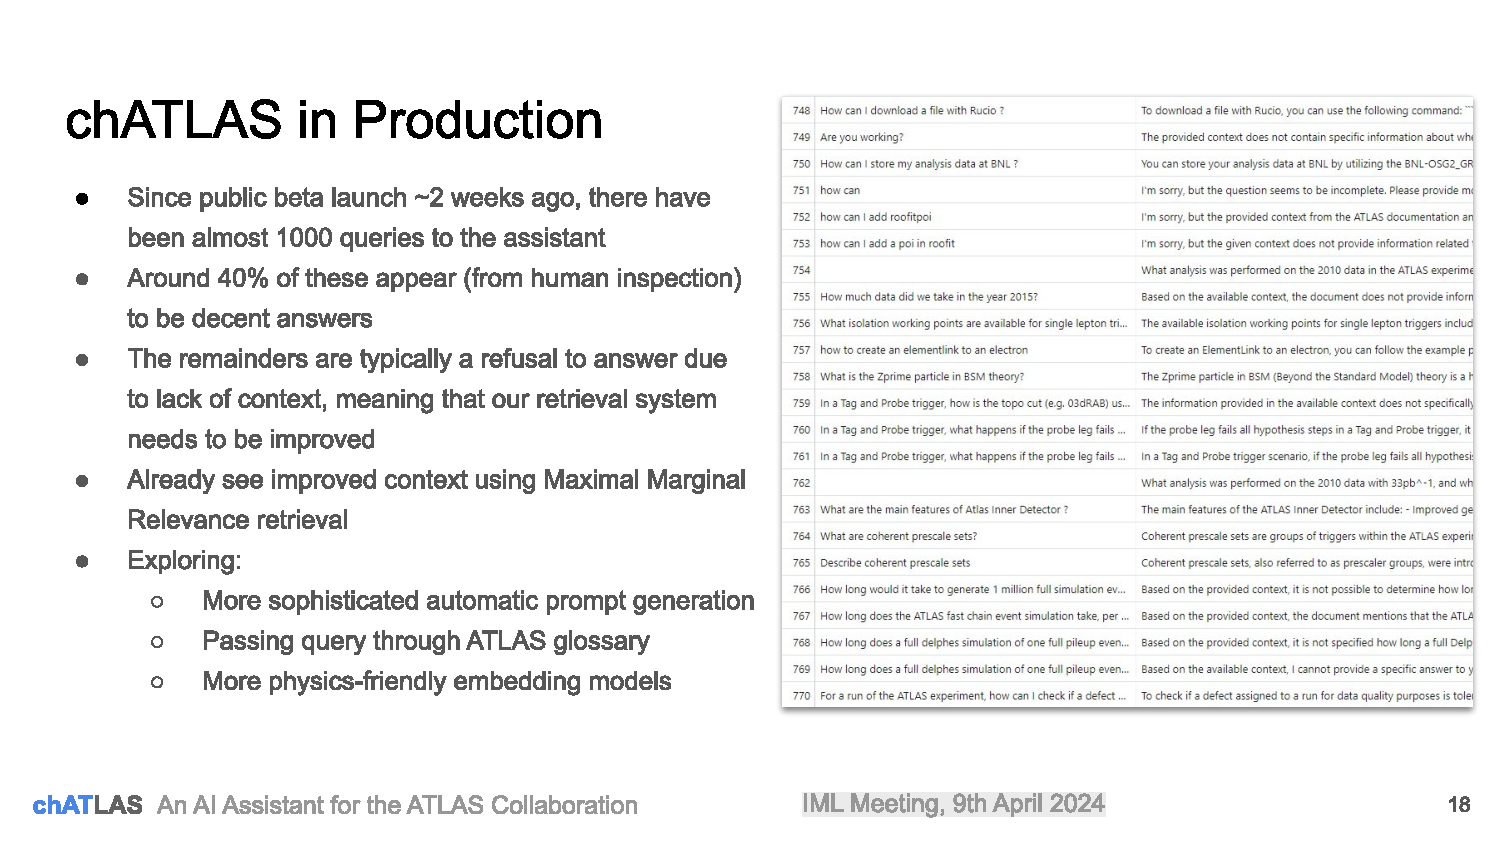
\includegraphics[width=0.94\linewidth]{PLOTS/chATLAS-40-percent-page18.pdf}}
\end{center}
\end{frame}

\begin{frame}{I started this March: {\bf \url{https://hep-help.org}}}
\vspace{0.25 cm}
\begin{center}
\fbox{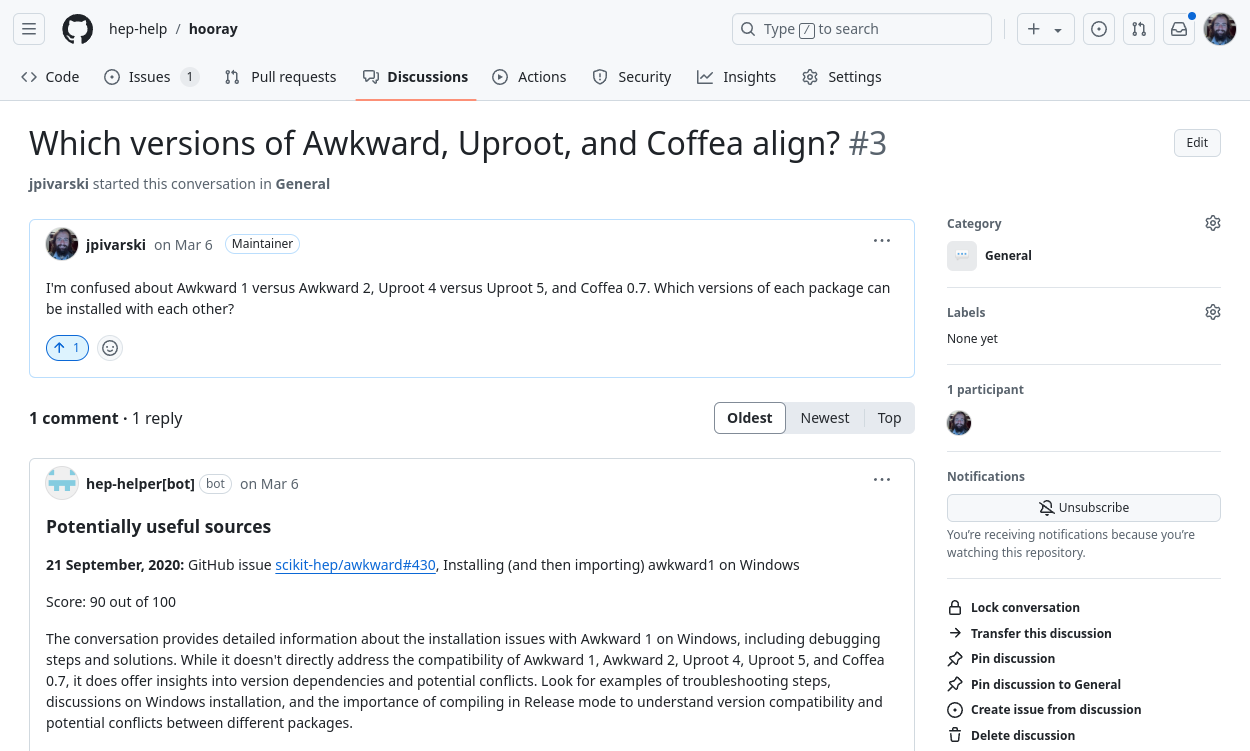
\includegraphics[width=0.87\linewidth]{PLOTS/hep-help-screenshot.png}}
\end{center}
\end{frame}

\begin{frame}{I'm sold on the user-interface choice}
\large
\vspace{0.35 cm}
GitHub Actions bot, wired into GitHub Discussions/Issues\ldots

\vspace{0.2 cm}
\begin{itemize}\setlength{\itemsep}{0.2 cm}
\item is free of charge and already has a nice UI (and CLI),
\item handles authentication and most of us already have accounts,
\item is not ephemeral/private: answered questions stay up for others to see,
\item can be commented on by humans (e.g.\ ``Careful! The above is wrong!''),
\item symmetrically cross-reference any GitHub issues/PRs they link to,
\item is implemented in GitHub Actions, which can run any code,
\item which can securely access secrets, such as an OpenAI API key.
\end{itemize}

\vspace{0.35 cm}
\uncover<2->{The response can take up to a minute, but compare that to a human responder.}

\vspace{0.35 cm}
\uncover<3->{Discussions or Issues? Discussions are threaded (3 levels) with up/down votes,}

\uncover<3->{\phantom{Discussions or Issues? }but Issues can ask users to fill out a structured form.}
\end{frame}

\begin{frame}[fragile]{How it works: using a CI workflow to respond to user posts}
\scriptsize
\vspace{-0.1 cm}
\begin{columns}[t]
\column{0.45\linewidth}
\begin{minted}{yaml}
name: answer-query
on:
  discussion:
    types: [created, edited]

jobs:
  answer-query:
    name: answer-query
    runs-on: ubuntu-latest
    steps:
      - name: Git checkout
        uses: actions/checkout@v4
        with:
          fetch-depth: 0
      - name: Get Python
        uses: actions/setup-python@v5
        with:
          python-version: "3.11"
      - name: Install dependencies
        run: |
          python -m pip install \
                 -r requirements.txt
\end{minted}

\column{0.65\linewidth}
\begin{minted}{yaml}
- name: Get vector store
  shell: bash
  run: |
    export TAG=`git describe --abbrev=0 --tags`
    wget https://github.com/hep-help/hooray/ \
         releases/download/$TAG/hep-help-db.zip
    unzip hep-help-db.zip
- name: Produce response
  shell: bash
  env:
    OPENAI_API_KEY: ${{ secrets.OPENAI_API_KEY }}
    BODY: ${{ github.event.discussion.body }}
  run: |
    echo "$BODY" | python answer-query.py > ./text.md
- name: Post response
  shell: bash
  env:
    APP_PRIVATE_KEY: ${{ secrets.APP_PRIVATE_KEY }}
    DISCUSSION_ID: ${{ github.event.discussion.node_id }}
  run: |
    echo "$APP_PRIVATE_KEY" > ./key.pem
    python comment-on-discussion.py
\end{minted}
\end{columns}
\end{frame}

\begin{frame}{What remains to be done}
\Large
\vspace{1 cm}

\setlength\fboxrule{1 pt}

\fcolorbox{white}{white}{\parbox{\textwidth}{\begin{itemize}
\item Gather documents from many sources: GitHub/GitLab, Slack, (public?) Mattermost, Gitter, StackOverflow, Discord\ldots
\end{itemize}}}

\vspace{0.3 cm}
\begin{onlyenv}<1>
\fcolorbox{white}{white}{\parbox{\textwidth}{\begin{itemize}
\item Understand how LLM technology works to improve responses
\end{itemize}}}
\end{onlyenv}\begin{onlyenv}<2>
\fbox{\parbox{\textwidth}{\begin{itemize}
\item Understand how LLM technology works to improve responses
\end{itemize}}}
\end{onlyenv}

\fcolorbox{white}{white}{\parbox{\textwidth}{\begin{itemize}
\item Streamline the user interface
\end{itemize}}}

\vspace{0.4 cm}
\fcolorbox{white}{white}{\parbox{\textwidth}{\begin{itemize}
\item Advertise widely
\end{itemize}}}

\vspace{-2.5 cm}
\hfill \uncover<2>{(the rest of this talk)}
\vspace{2.5 cm}
\end{frame}

\begin{frame}{Possible workflow \only<1>{\#1}\only<2>{\#2}\only<3>{\#3 (what hep-help currently does)}\only<4>{\#4}\only<5>{\#5}}
\Large
\vspace{0.5 cm}
\begin{columns}
\column{1.1\linewidth}
\only<1>{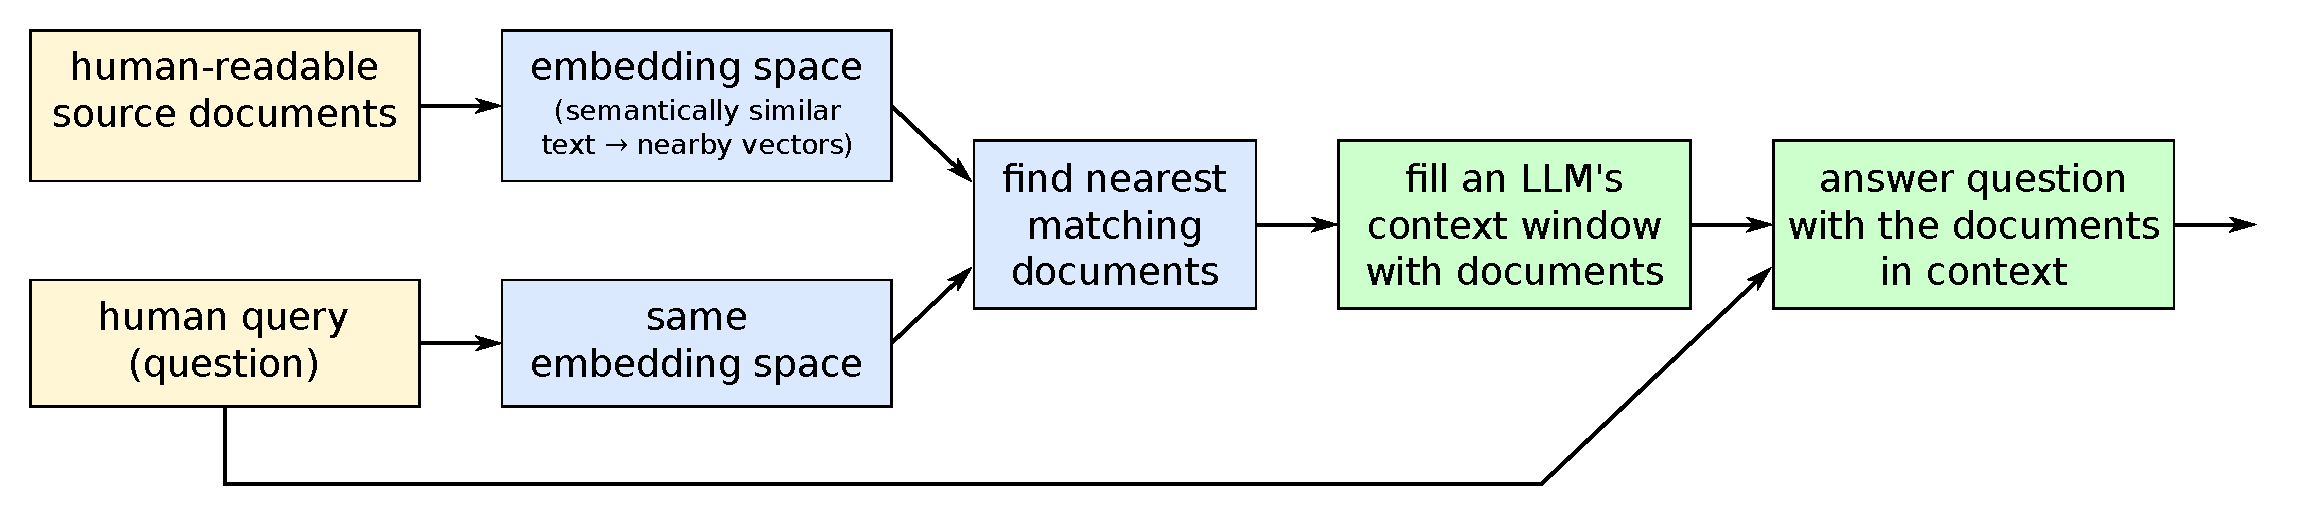
\includegraphics[width=\linewidth]{PLOTS/explain-rag-1.pdf}}\only<2>{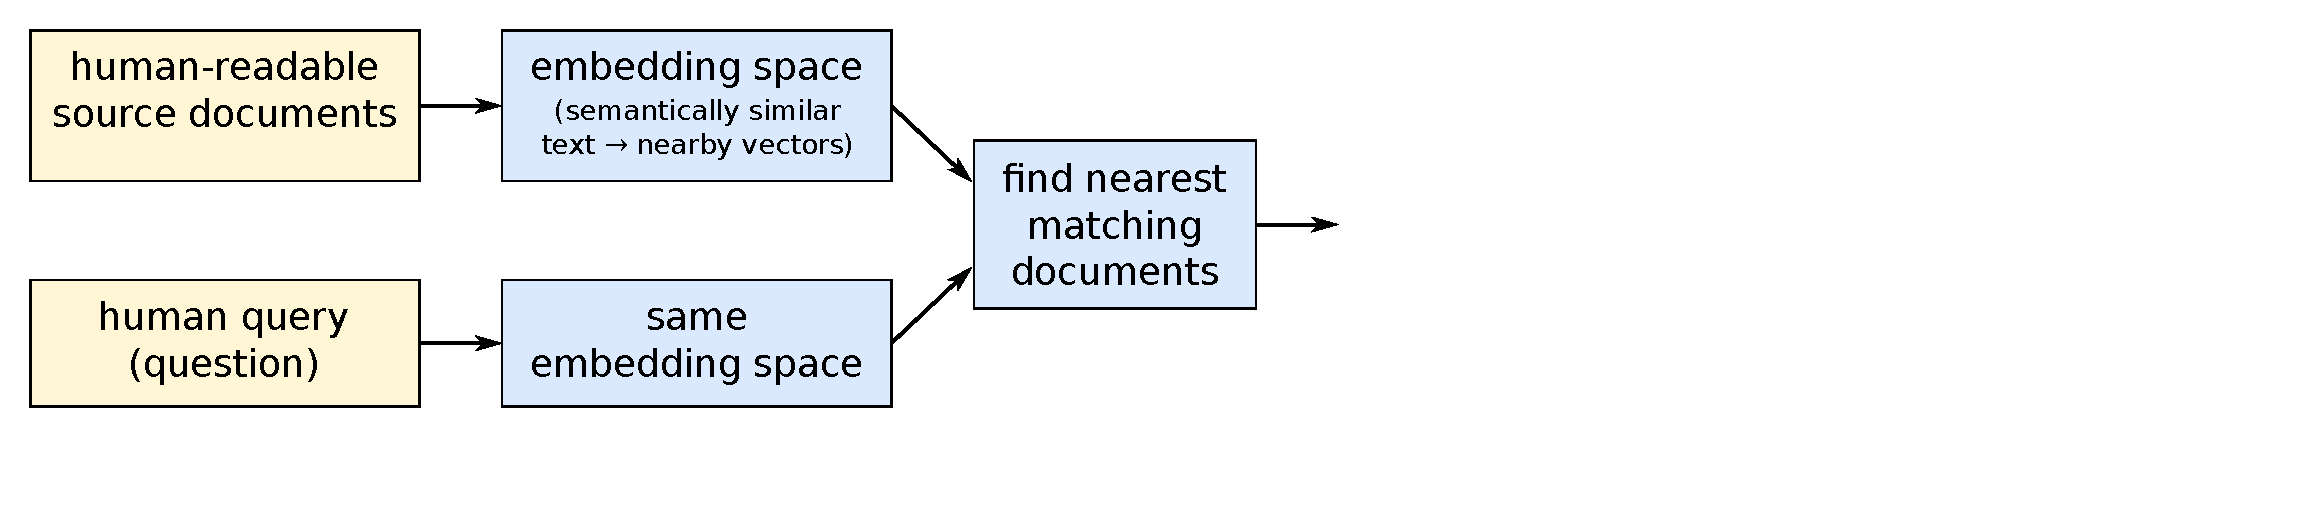
\includegraphics[width=\linewidth]{PLOTS/explain-rag-2.pdf}}\only<3>{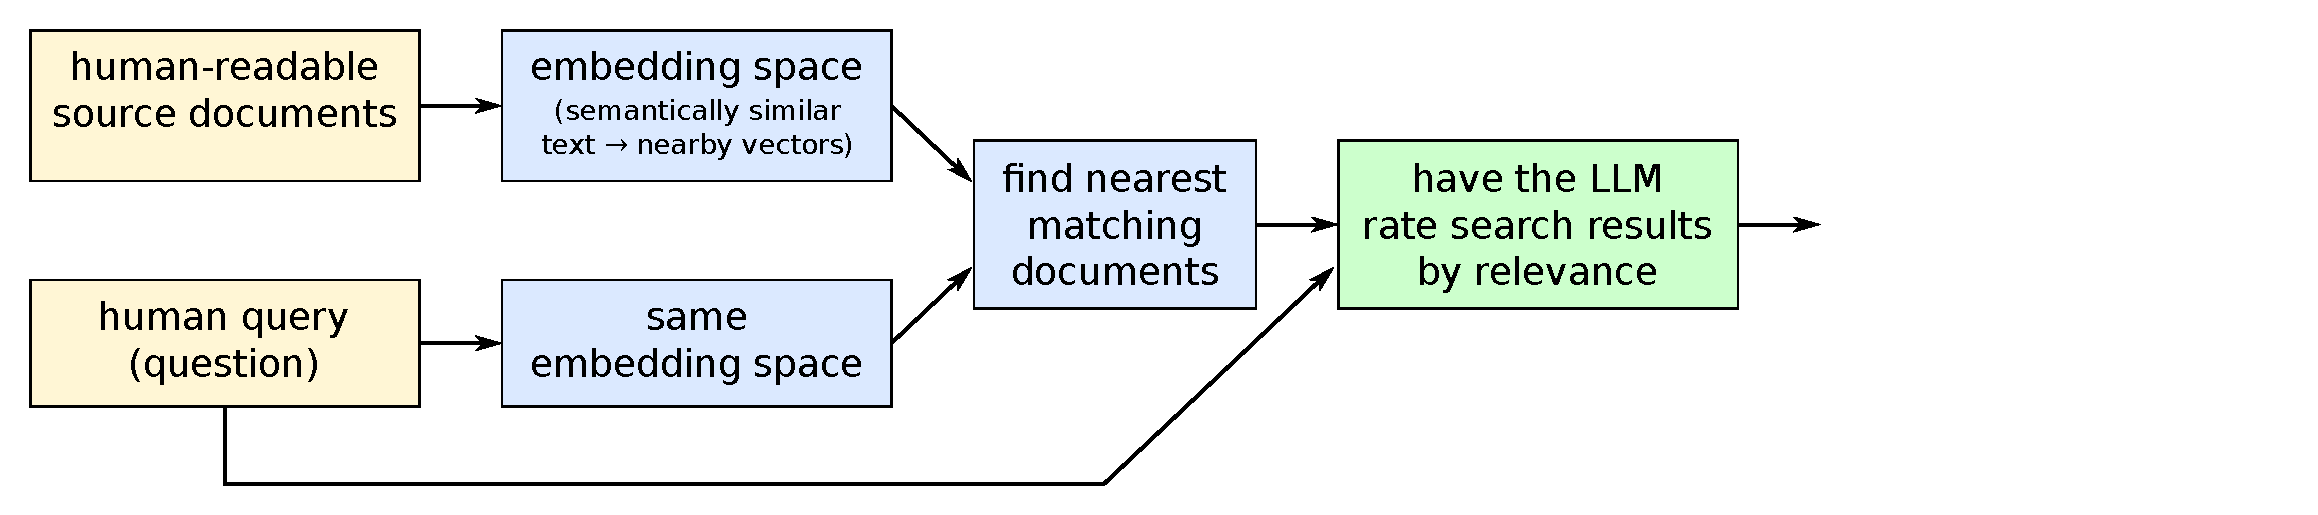
\includegraphics[width=\linewidth]{PLOTS/explain-rag-3.pdf}}\only<4>{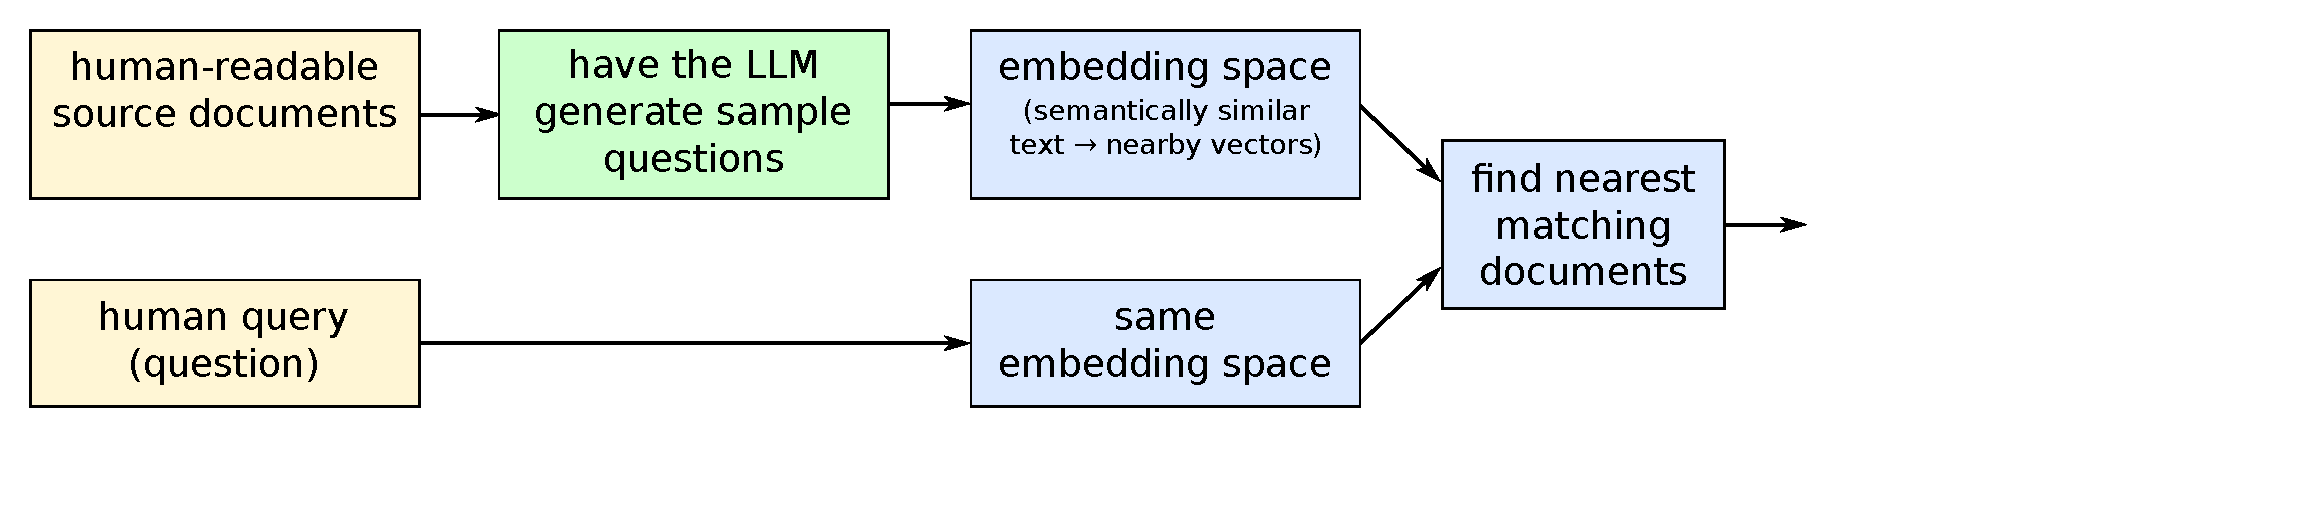
\includegraphics[width=\linewidth]{PLOTS/explain-rag-4.pdf}}\only<5>{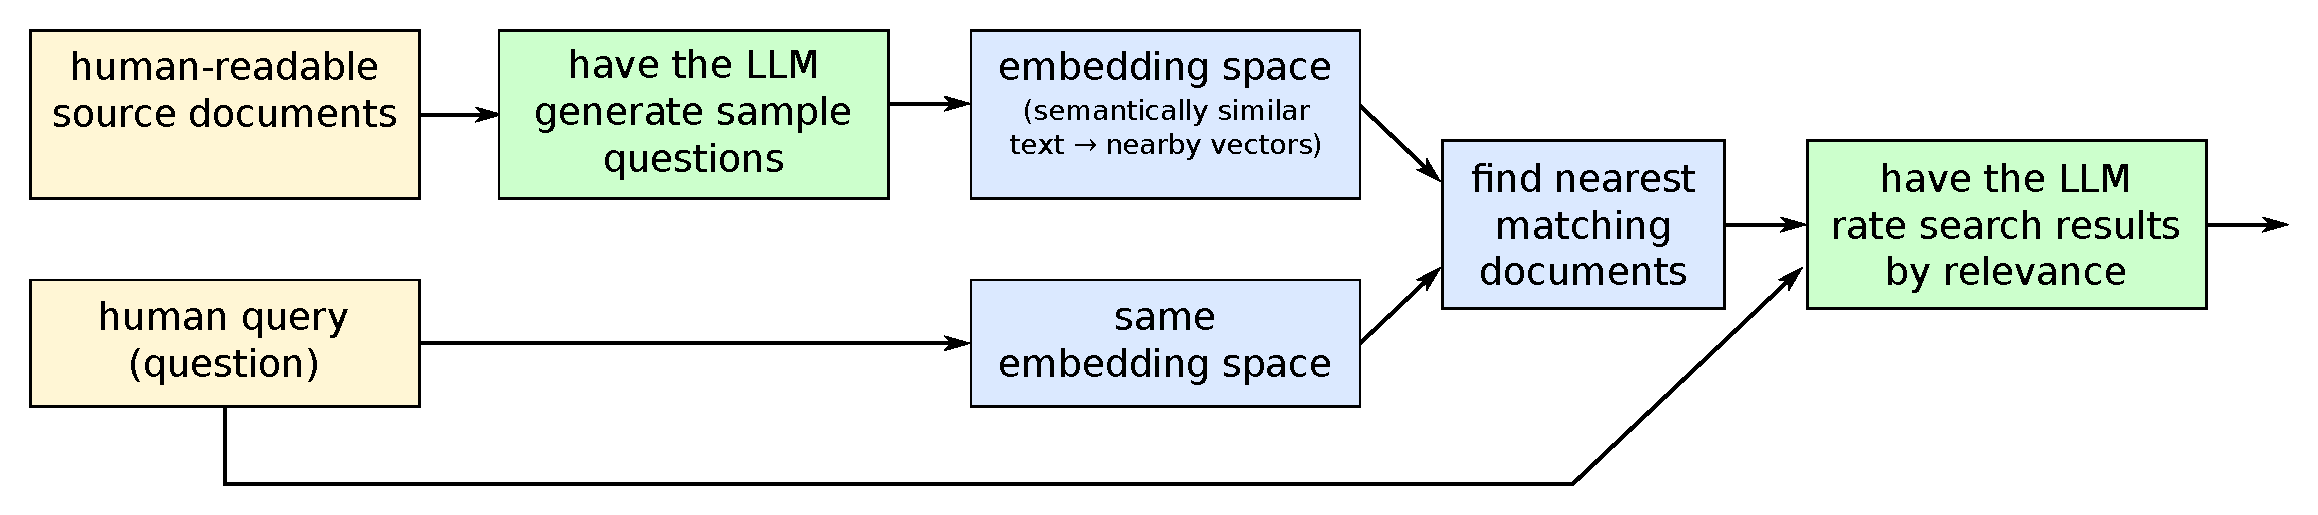
\includegraphics[width=\linewidth]{PLOTS/explain-rag-5.pdf}}
\end{columns}

\vspace{0.5 cm}
\begin{onlyenv}<1>
\textcolor{darkblue}{Retrieval-Augmented Generation (RAG):}

\large
\vspace{0.25 cm}
An LLM is better able to answer questions if it has relevant information in its (limited-size) context window.

\vspace{0.25 cm}
Get information by passing documents and query through the same neural network; in that embedding space, similar vectors are semantically similar text.

\vspace{10 cm}
\end{onlyenv}\begin{onlyenv}<2>
\textcolor{darkblue}{Just semantic search:}

\large
\vspace{0.25 cm}
Maybe we don't need the LLM at all! If we can match a query to semantically similar documents, perhaps we should just recommend these documents.

\vspace{10 cm}
\end{onlyenv}\begin{onlyenv}<3>
\textcolor{darkblue}{Semantic search with re-ranking:}

\large
\vspace{0.25 cm}
Some embedding space matches aren't actually related to the query, even though they touch on the same concepts.

\vspace{0.25 cm}
Use the LLM in a limited way: have it rate and describe how relevant each match is to the human query.

\vspace{10 cm}
\end{onlyenv}\begin{onlyenv}<4>
\textcolor{darkblue}{Better targets in embedding space:}

\large
\vspace{0.25 cm}
The human query is a question, and a question is a better semantic match to a question than an answer to that question.

\vspace{0.25 cm}
Use the LLM in a limited way: have it generate possible questions about the source documents.

\vspace{10 cm}
\end{onlyenv}\begin{onlyenv}<5>
\textcolor{darkblue}{Combine \#3 and \#4:}

\large
\vspace{0.25 cm}
Note: the LLM cost for \#3 scales with the number of documents, but

\phantom{Note: the LLM cost for }\#4 scales with the number of human queries.
\vspace{10 cm}
\end{onlyenv}
\end{frame}

\begin{frame}{Without a good embedding, we won't find the right documents}
\vspace{0.5 cm}
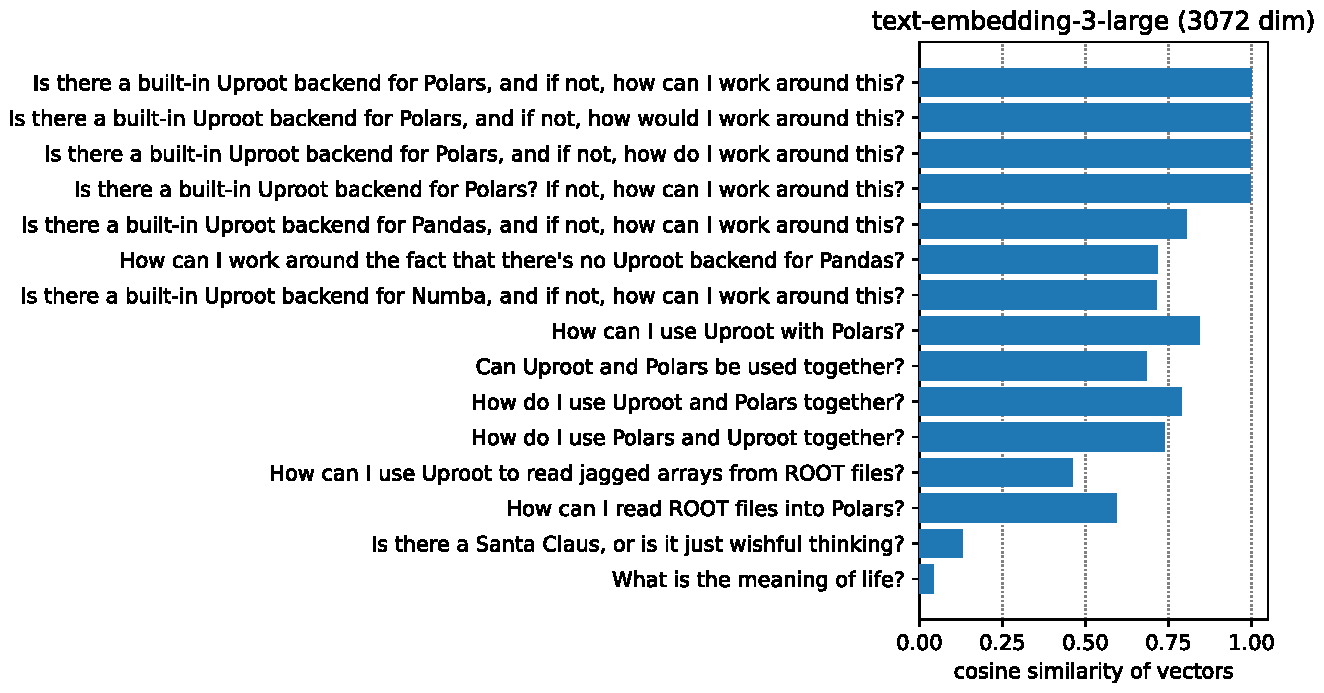
\includegraphics[width=\linewidth]{PLOTS/experiments-with-similarity.pdf}

\vspace{-0.75 cm}
\textcolor{darkblue}{So this is the most important thing to understand.}
\vspace{0.75 cm}
\end{frame}

\begin{frame}{How much wiggle room is there between signal and background?}
\large
\vspace{0.5 cm}
Consecutive Slack messages (IRIS-HEP Slack) are a large sample of question-answer pairs. Non-consecutive ones are ``background.''

\vspace{0.25 cm}
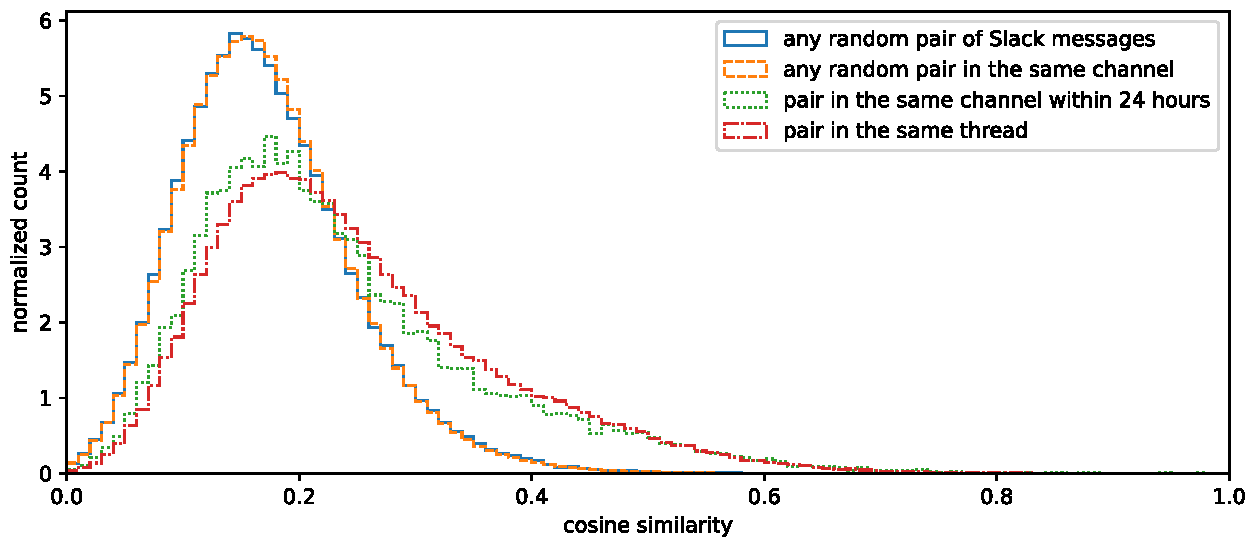
\includegraphics[width=\linewidth]{PLOTS/slack-similarity-in-and-out-of-threads.pdf}
\end{frame}

\begin{frame}{Cleaner set of question-answer pairs: StackOverflow}
\vspace{0.25 cm}
\begin{center}
\fbox{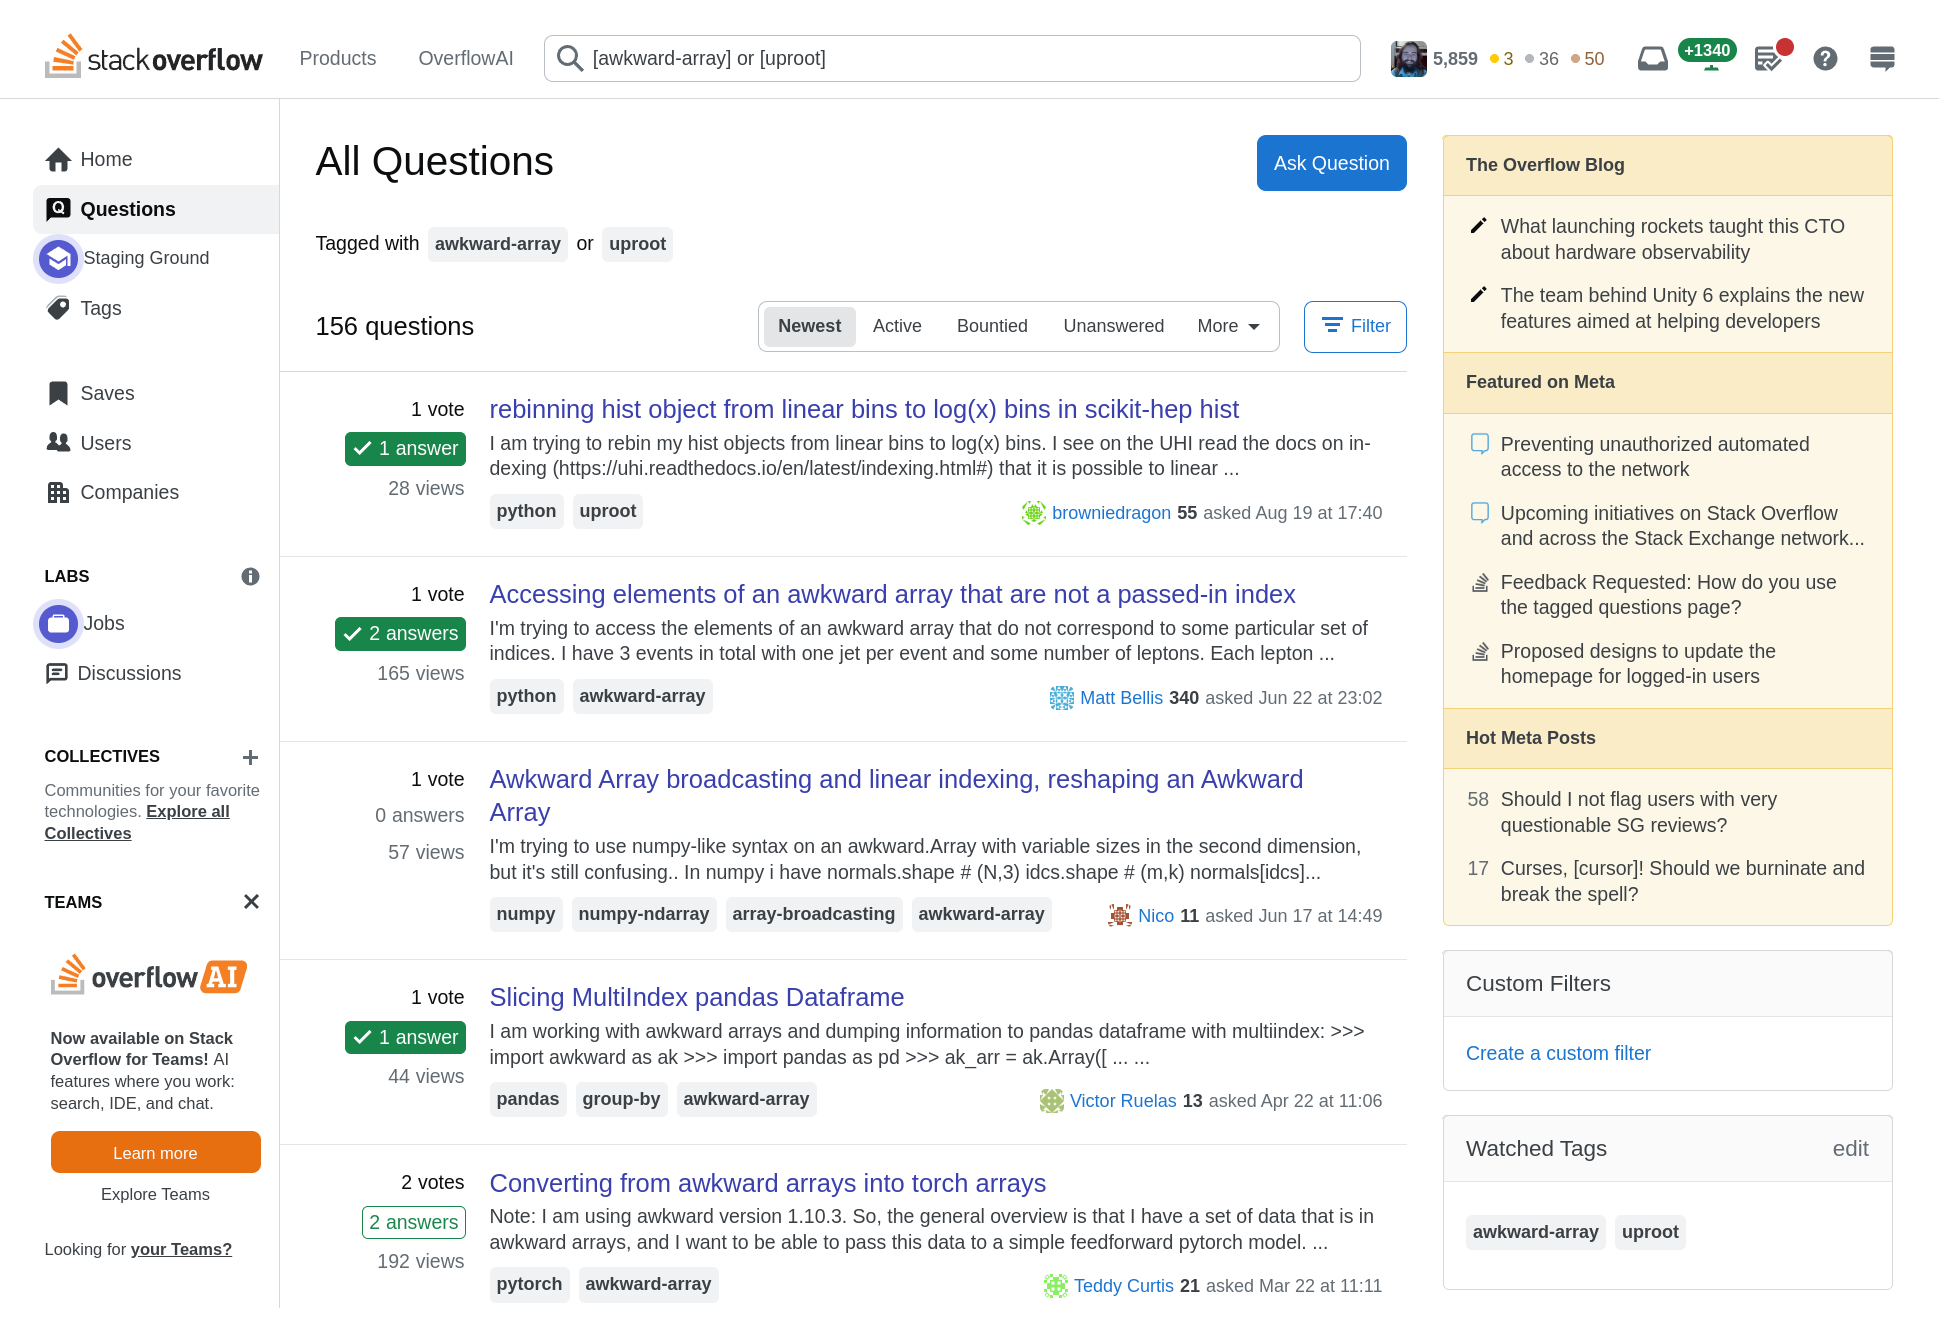
\includegraphics[width=0.76\linewidth]{PLOTS/stackoverflow-screenshot.png}}
\end{center}
\end{frame}


\end{document}
